\documentclass{article}
\usepackage{tikz}

\begin{document}

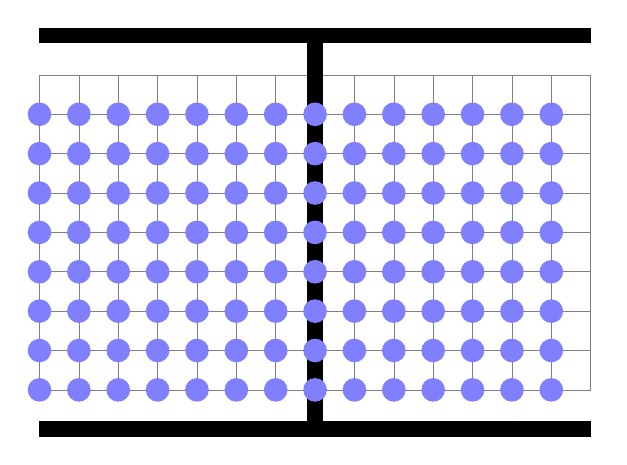
\begin{tikzpicture}[scale=0.5]
    % Draw the grid lines
    \draw[help lines] (0,0) grid (14,8);
    
    % Draw the vertical black line
    \draw[line width=2mm, color=black] (7,-1) -- (7,9);
    
    % Draw the horizontal black line at the bottom
    \draw[line width=2mm, color=black] (0,-1) -- (14,-1);
    
    % Draw the horizontal black line at the top
    \draw[line width=2mm, color=black] (0,9) -- (14,9);
    
    % Draw the blue circles
    \foreach \x in {0,...,13} {
        \foreach \y in {0,...,7} {
            \fill[blue!50] (\x,\y) circle (0.3);
        }
    }
\end{tikzpicture}

\end{document}